\documentclass[wide,a4paper,titlepage,12pt] {article}
\usepackage{polski}
\usepackage[utf8]{inputenc}
\usepackage{listings}
\usepackage{slashbox}
\usepackage[table]{xcolor}
\usepackage{graphicx,pdflscape}
\usepackage{placeins}

\title{Projektowanie efektywnych algorytmów}
\author{Tymon Tobolski (181037)\\ Jacek Wieczorek (181043)}

% Title page layout (fold)
\makeatletter
\renewcommand{\maketitle}{
\begin{titlepage}
  \begin{center}
    \vspace*{3cm}
    \LARGE \@title \par
    \vspace{2cm}
    \textit{\small Autor:}\par
    \normalsize \@author\par \normalsize
    \vspace{3cm}
    \textit{\small Prowadzący:}\par
   Prof. dr hab. inż Adam Janiak \par
    \vspace{2cm}
    Wydział Elektroniki\\ III rok\\ Cz TN 13.15 - 15.00\par
    \vspace{4cm}
    \small \@date
  \end{center}
\end{titlepage}
}
\makeatother

\begin{document}
\maketitle
  \section{Cel projektu}
\paragraph{}
Celem projketu jest zaimplementowanie i przetestowanie metaheurystycznego algorytmu symulowanego wyżarzania dla porblemu szeregowania zadań na jednym procesorze przy kryterium minimalizacji wazonej sumy opóźnień zadań.
  \section{Opis problemu}
{\bf Jednoprocesorowy problem szeregowania zadań przy kryterium
minimalizacji ważonej sumy opóźnień zadań.}
\paragraph{}
Danych jest $n$ zadań (o numerach od 1 do $n$), które mają być wykonane bez przerwań przez pojedynczy procesor, mogący wykonywać co najwyżej jedno zadanie jednocześnie.
Każde zadanie j jest dostępne do wykonania w chwili zero, do wykonania wymaga $p_{j} > 0$ jednostek czasu oraz ma określoną wagę (priorytet) $w_{j} > 0$ i oczekiwany termin zakończenia
wykonywania $d_{j} > 0$. Zadanie $j$ jest spóźnione, jeżeli zakończy się wykonywać po swoim terminie $d_{j}$, a miarą tego opóźnienia jest wielkość $T_{j} = max(0, C_{j} - d_{j} )$, gdzie $C_{j}$ jest terminem zakończenia
wykonywania zadania $j$. Problem polega na znalezieniu takiej kolejności wykonywania zadań (permutacji) aby zminimalizować kryterium $TWT = \Sigma_{j=1}^{n} w_{j} T_{j}$.
\section{Opis algorytmu}
\paragraph{}
Symulowane wyżarzanie to algorytm heurystyczny przeszukującego przestrzeń alternatywnych rozwiązań problemu w celu wyszukania rozwiązań najlepszych. Sposób działania algorytmu jest analogią do zjawiska wyżarzania w metalurgii.
\paragraph{}
Przebieg algorytmu :
\begin{enumerate}
  \item Wybranie losowego punktu startowego $\omega$ i przypisanie $T = T_{max}$
  \item Wyznaczenie wartości $F(\omega)$
  \item 
\end{enumerate}	
\section{Implementacja}
Jezykiem implementacji algorytmu jest $Scala$ w wersji $2.9.1$ działająca na $JVM$. \\
TODO jakies lsitingi itp
\section{Testy}
\paragraph{}
Testy algorytmu symulowanego wyżarzania przeprowadzone zostały dla trzech zestawów testów o róznym rozmiarze porblemu $n$, każdy składający się ze 125 instancji. Parametry podstawowe jak $T_{min}$ i $T_{max}$ w przypadku każdego testu były takie same. Zmieniany natomiast był parametr $T_{d}$.
\paragraph{}
Jako wyniki testów przedstawiamy zsumowany czas liczenia wszystkich instancji dla danego rozmiaru problemu, a także sumę błedów względnych njalepszych rozwiązań dla każdej instancji. 
\paragraph{}
Parametry niezmienne : 
\begin{itemize}
  \item $T_{min} = 0.01$
  \item $T_{max} = 100$
\end{itemize}
\newpage
\subsection{n = 40}
\begin{center}
    \begin{tabular}{|c|c|c|}
      \hline
       $T_{d}$ & Time & Difference \\ \hline
       0,99 & 5,78 & 27,41 \\ \hline
       0,999 & 46,26 & 2,52 \\ \hline
       0,9999 & 434,52 & 0,43 \\ \hline
  \end{tabular}
\end{center}

\begin{figure}[htbp]
  \begin{center}
         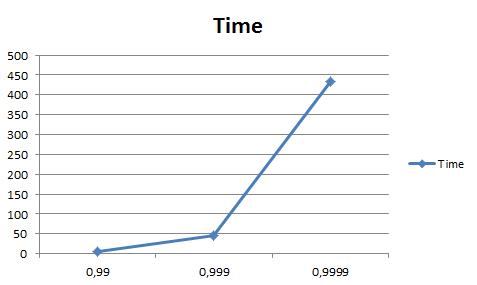
\includegraphics[scale=0.8]{time40.PNG}
         \caption{Czas rozwiązywania w zależności od parametru $T_d$}
  \end{center}
\end{figure}

\begin{figure}[htbp]
  \begin{center}
         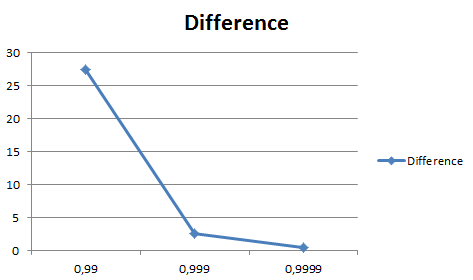
\includegraphics[scale=0.8]{diff40.PNG}
         \caption{Błąd względny rozwiązywania w zależności od parametru $T_d$}
  \end{center}
\end{figure}

\newpage
\subsection{n = 50}
\begin{center}
    \begin{tabular}{|c|c|c|}
      \hline
       $T_{d}$ & Time & Difference \\ \hline
       0,99 & 6,63 & 169,02 \\ \hline
       0,999 & 53,09 &8,47 \\ \hline
       0,9999 & 519,04 & 0,95 \\ \hline
  \end{tabular}
\end{center}

\begin{figure}[htbp]
  \begin{center}
         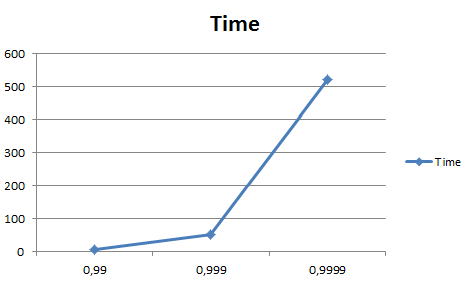
\includegraphics[scale=0.8]{time50.PNG}
         \caption{Czas rozwiązywania w zależności od parametru $T_d$}
  \end{center}
\end{figure}

\begin{figure}[htbp]
  \begin{center}
         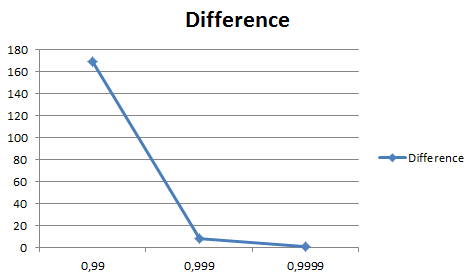
\includegraphics[scale=0.8]{diff50.PNG}
         \caption{Błąd względny rozwiązywania w zależności od parametru $T_d$}
  \end{center}
\end{figure}

\newpage
\subsection{n = 100}
\begin{center}
    \begin{tabular}{|c|c|c|}
      \hline
       $T_{d}$ & Time & Difference \\ \hline
       0,99 & 12,4 & 579,97 \\ \hline
       0,999 & 104,18 & 23,43 \\ \hline
       0,9999 & 990 & 3,42 \\ \hline
  \end{tabular}
\end{center}

\begin{figure}[htbp]
  \begin{center}
         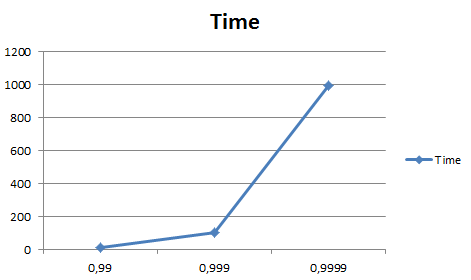
\includegraphics[scale=0.8]{time100.PNG}
         \caption{Czas rozwiązywania w zależności od parametru $T_d$}
  \end{center}
\end{figure}

\begin{figure}[htbp]
  \begin{center}
         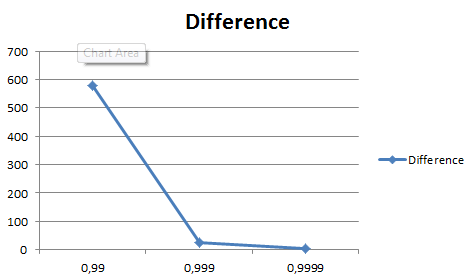
\includegraphics[scale=0.8]{diff100.PNG}
         \caption{Błąd względny rozwiązywania w zależności od parametru $T_d$}
  \end{center}
\end{figure}
\newpage
\subsection{Porównanie wszytskich zadań}
\begin{figure}[htbp]
  \begin{center}
         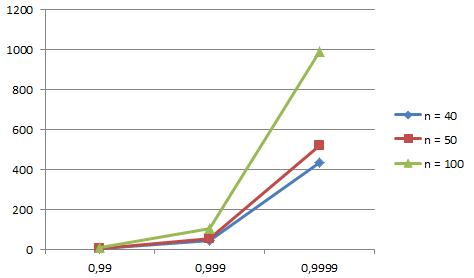
\includegraphics[scale=0.8]{complexTime.PNG}
         \caption{Czas rozwiązywania w zależności od parametru $T_d$}
  \end{center}
\end{figure}

\begin{figure}[htbp]
  \begin{center}
         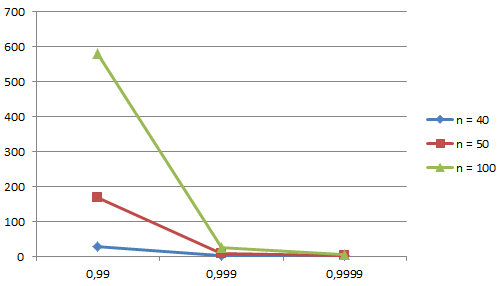
\includegraphics[scale=0.8]{complexDiff.PNG}
         \caption{Błąd względny rozwiązywania w zależności od parametru $T_d$}
  \end{center}
\end{figure}
\newpage
\section{Wnioski}
\end{document}



